% Canonical paper source for the stage-1 iRoute monorepo refactor.
\documentclass[journal]{IEEEtran}

\usepackage{cite}
\usepackage{amsmath,amssymb,amsfonts}
\usepackage{algorithmic}
\usepackage{algorithm}
\usepackage{graphicx}
\usepackage{textcomp}
\usepackage{xcolor}
\usepackage{bm}
\usepackage{booktabs}
\usepackage{multirow}
\usepackage{url}
\usepackage{subcaption}
\usepackage{pifont}
\usepackage{tabularx}
\usepackage{array}
\usepackage{tikz}

\newcommand{\sysname}{iRoute}
\newcommand{\PSDC}{\texttt{ParametersSha256Digest\allowbreak Component}}
\newcommand{\AP}{\texttt{Application\allowbreakParameters}}
\newcommand{\boldparagraph}[1]{\vspace{0.1cm}\noindent\textbf{#1.}}
\def\BibTeX{{\rm B\kern-.05em{\sc i\kern-.025em b}\kern-.08em
    T\kern-.1667em\lower.7ex\hbox{E}\kern-.125emX}}
% === end iRoute additions ===

\begin{document}

\title{iRoute: Semantic Discovery for Interoperable NDN-IoT under Naming Heterogeneity}

\author{}

\markboth{}%

\maketitle

\begin{abstract}
Internet-of-Things (IoT) deployments increasingly span multiple administrative domains and integrate heterogeneous vendors and vertical applications. Service access is therefore often intent-driven: consumers describe the desired sensing data or service semantics, yet lack precise knowledge of each producer's naming convention. Baseline Named Data Networking (NDN) relies on exact name matching and longest-prefix forwarding over hierarchical strings; under heterogeneous and transient IoT namespaces, this assumption frequently causes discovery failures and drives the growth of forwarding and control-plane state.

This paper presents \sysname{}, a bounded-state semantic discovery and routing framework for NDN-enabled IoT interoperability. \sysname{} decouples inference from delivery via a two-stage workflow: an ingress gateway issues semantic discovery Interests that remain topologically routable while carrying an intent vector, and a subsequent fetch Interest retrieves the resolved canonical name or manifest using unmodified NDN forwarding. To bound routing-plane scalability costs, \sysname{} enforces a hard advertisement budget: each domain exports only a fixed number of semantic centroids as its external summary, limiting disseminated semantic state while preserving compatibility with longest-prefix matching in the core. We evaluate \sysname{} in ndnSIM on representative multi-domain IoT settings with heterogeneous naming, and show improved discovery success with reduced control overhead and bounded routing state.
\end{abstract}

\begin{IEEEkeywords}
Named Data Networking, Internet of Things, smart city, heterogeneous naming, semantic routing, bounded routing state
\end{IEEEkeywords}

\IEEEpeerreviewmaketitle


\section{Introduction}
\label{sec:introduction}

Smart-city IoT deployments increasingly operate as federations of independently managed subsystems such as transportation, environmental monitoring, utilities, and public safety, which are often owned and operated by different agencies and vendors. A recurring access pattern in these environments is intent-driven service access: applications describe the desired information in terms of semantics and context, for example, recent congestion conditions in a given downtown area or PM2.5 alerts within a specific district, while lacking precise knowledge of the naming convention adopted by each subsystem. In practice, semantically equivalent resources are frequently published under heterogeneous hierarchical names that differ in structure and terminology due to legacy systems, vendor-specific identifiers, and evolving service lifecycles, which makes interoperability at the edge particularly brittle.

Named Data Networking (NDN)~\cite{ndn} is a natural substrate for smart-city IoT because it replaces host addresses with names, enables in-network caching, and supports data-centric security. However, elevating application-layer names to the network layer introduces a fundamental tension between expressiveness and scalability. An NDN name simultaneously serves as an application identifier (describing what the data/service is) and as a network locator (guiding Interests toward where it resides). While smart-city applications demand rich, dynamic, and heterogeneous namespaces to capture semantics and context, the routing system requires bounded, stable, and aggregatable prefixes for global scalability. Baseline NDN forwarding thus implicitly assumes that consumers can issue Interests matching producer-exposed names and that routing can aggregate those names into a manageable set of prefixes for longest-prefix matching.

Under heterogeneous and transient smart-city namespaces, this assumption breaks down: exact name matching can fail even when the network hosts semantically relevant data, and maintaining reachability by enumerating finer-grained prefixes pressures the network to disseminate and store an ever-growing set of disjoint forwarding entries~\cite{inf_ndn_iot}. This creates a ``syntactic cliff'': the richer and more diverse the namespace becomes, the harder it is for the network to remain both interoperable and scalable. In operational smart-city stacks, bridging this gap often falls back to out-of-band resolution mechanisms, such as subsystem-specific service catalogs, centralized registries, or keyword-based portals that map intents to canonical names. These mechanisms reduce immediate failures, but they reintroduce centralized dependencies, impose cross-agency naming coordination, and ultimately move ``name discovery'' outside the network layer, weakening the end-to-end simplicity that name-based communication aims to provide.

Existing NDN-IoT efforts partially address this tension but leave a key routing-plane question unresolved. Hybrid naming schemes support multiple IoT object types and mitigate ambiguity, but still require convention alignment and do not prevent namespace-driven state growth~\cite{hybrid_iot_naming}. Semantic-assisted forwarding can recover from exact-match failures by performing semantic matching (often at the edge), yet it typically does not provide a network-wide bounded-state abstraction for cross-domain discovery~\cite{semantic_name_forwarding_iotmag25}. Semantic-aware naming resolution and caching further show that exact-match policies overlook semantic relationships important to IoT workloads, but these improvements primarily target local resolution or cache efficiency rather than routing-plane scalability~\cite{sanr_cmf}. Together, these lines of work motivate a missing capability: cross-domain semantic discovery that remains compatible with core longest-prefix forwarding while keeping disseminated routing state bounded.

This paper presents \sysname{}, a bounded-state semantic discovery and routing framework that targets smart-city interoperability across domains. The key observation is that semantic locality in smart-city IoT is often domain-scoped: each subsystem or administrative domain typically hosts coherent collections of services and data types, even if internal names remain heterogeneous. \sysname{} leverages this structure by allowing each domain to summarize its internal namespace into a fixed number of semantic centroids under a hard advertisement budget. These centroids serve as externally disseminated semantic summaries, enabling intent-driven discovery while bounding exported routing state independent of the number of internal objects.

\sysname{} decouples inference from delivery via a two-stage workflow. An ingress gateway issues a semantic discovery Interest that remains topologically routable by placing a destination domain prefix first, while carrying an intent vector in \AP. Discovery forwarding uses lightweight similarity-aware decision rules to probe a small set of candidate domains without requiring core routers to interpret application semantics. After discovery resolves a routable pointer (a canonical name or a manifest prefix), the consumer retrieves the content using a standard fetch Interest under unmodified NDN forwarding and caching. This separation preserves compatibility with longest-prefix matching in the core and keeps semantic computation off the critical path of data delivery.

In summary, \sysname{} contributes a domain-level semantic summarization interface with a strict advertisement budget to bound routing state under smart-city naming heterogeneity, a compatible discovery-and-delivery protocol that enables intent-driven service access without assuming a unified naming convention, and an end-to-end design connecting control-plane advertisement, similarity-aware discovery forwarding, and canonical-name retrieval in a deployable NDN-IoT setting. The remainder of this paper is organized as follows. Section~\ref{sec:background} reviews the background and motivates bounded-state semantic interoperability in NDN-IoT. Section~\ref{sec:design} presents the architecture and design of \sysname{}. Section~\ref{sec:spec} specifies the protocol and implementation details. Section~\ref{sec:eval} evaluates \sysname{} under representative heterogeneous smart-city settings, followed by discussion and limitations.

% =============================================================================
\section{Background and Motivation}
\label{sec:background}
% =============================================================================

IoT interoperability challenges are often rooted in naming.
In smart-city deployments, semantically equivalent signals or service functions are routinely published under heterogeneous namespaces across subsystems, vendors, and administrative domains, while consumers frequently operate with only partial naming knowledge. This gap exposes a fundamental tension in name-based networking: applications require expressive, dynamic names to encode semantics and context, whereas routing demands bounded, stable, and aggregatable prefixes for scalability. When these goals are simultaneously imposed on hierarchical strings, deployments can hit a ``syntactic cliff'': intent-level requests are natural at the application layer, yet forwarding requires a routable canonical name, and bridging the mismatch either falls back to out-of-band directories or forces increasingly fine-grained prefix dissemination.

A promising alternative is to inject limited semantic awareness into the discovery process, so that the network can steer intent queries toward a small set of candidate domains that are likely to host relevant content. Importantly, the objective is not to replace name-based delivery, but to efficiently locate a routable pointer (a canonical name or a manifest prefix) that can be fetched with standard NDN forwarding. Realizing this capability in IoT settings requires addressing two constraints that are easy to overlook: semantic similarity is high-dimensional and non-hierarchical, which can trigger routing-state growth if mapped naively into forwarding tables, and semantic inference is compute-intensive, which conflicts with per-packet processing on resource-constrained paths. These constraints motivate iRoute's bounded-state, edge-assisted design.

\subsection{Named Data Networking}
\label{sec:bg_ndn}

NDN is an information-centric networking architecture where consumers retrieve data (or invoke services) by names rather than by host addresses. A consumer issues an \texttt{Interest} carrying a hierarchical name, routers forward it via longest-prefix matching (LPM) over the \texttt{FIB}, and the matching producer (or an in-network cache) returns a \texttt{Data} packet that follows the reverse path via \texttt{PIT} state. This receiver-driven exchange naturally supports multipath and anycast retrieval and enables in-network caching, which are desirable properties for IoT deployments with intermittent connectivity and repeated, localized queries.

Despite these advantages, interoperability remains challenging because the standard NDN data plane assumes that the requester knows a routable name (or prefix) that can be matched in the network. In IoT, this assumption is fragile: services and data streams are authored by heterogeneous devices and administrative domains, and names often embed transient attributes (location, time, device identifiers, sensor types) that vary across vendors. Consequently, semantically valid requests can fail purely due to syntactic mismatch, and strict prefix-based routing pressures systems toward alias enumeration, directory-style indirection, or flooding when consumers lack exact naming knowledge~\cite{amadeo2025saf,dt_vndn_semantic,grewe2018sodi}. Bridging naming heterogeneity without sacrificing scalability is therefore central to IoT interoperability over NDN.

We consider IoT deployments organized into administrative domains, each associated with a routable topological prefix (e.g., a smart-city subsystem, a campus or micro-operator edge, or an RSU cluster).
A domain hosts producers (devices, services, and caches) and is connected via one or more edge gateways that participate in control and discovery.
The problem studied in this paper is to map an intent query to a relevant canonical name (or manifest) in a multi-domain setting, while avoiding global indexing and keeping semantic inference off the core forwarding path.

\subsection{Semantic IoT Interoperability}
\label{sec:bg_semantic_iot}

A substantial body of IoT-oriented work recognizes that exact string matching is an overly rigid interface between applications and the network, and introduces semantic models to tolerate naming mismatch. One common approach is to enrich service discovery with contextual and semantic descriptions, so that requests can be matched to device capabilities or service functions even when names are inconsistent across vendors. For example, contextual IoT service discovery evaluates semantic models and similarity mechanisms for flexible matching over heterogeneous device descriptions~\cite{antunes2022context}. Such efforts clarify the need for query-by-intent interfaces, but they typically assume the existence of a discovery index, directory, or knowledge base, and their decentralization and control overhead depend on how that index is provisioned and maintained.

Another line of work injects semantics into the naming and name distribution pipeline. Hybrid naming schemes attempt to unify naming for different IoT object types (content, devices, and services) and reduce ambiguity, while acknowledging the practical constraints of IoT deployments such as variable-length names and resource-limited devices~\cite{hybrid_iot_naming}. Other proposals study semantic-driven name distribution and retrieval mechanisms that leverage semantic relationships to assist lookup and dissemination. These designs improve expressiveness and matching flexibility, but they do not by themselves provide a bounded inter-domain reachability abstraction; without explicit controls, disseminated state and update traffic can still scale with namespace diversity.

Overall, semantic IoT proposals motivate a clear principle for routing and discovery: semantic matching should improve robustness to naming heterogeneity, but it must be coupled with a scalability mechanism that bounds exported state and avoids heavy per-packet inference on constrained paths. This motivates iRoute's focus on the routing and discovery interface, where domains export compact semantic summaries under an explicit budget.

\subsection{Related Work}
\label{sec:bg_related}

Semantic support for NDN-based IoT has been studied across multiple layers of the protocol stack, largely motivated by interoperability under naming heterogeneity.
A recurring observation is that IoT applications issue intent-level requests while producers expose functionally equivalent resources under inconsistent namespaces, whereas the forwarding substrate is optimized for exact name-prefix operations.
Existing designs therefore differ mainly in where semantic signals are introduced and how they trade robustness to naming mismatch against state, compute, and control overhead.

\textbf{Routing-plane approaches.}
A first class of systems retains standard forwarding and focuses on disseminating reachability information.
Conventional NDN routing (e.g., NLSR) advertises exact prefixes and thus inherits the scalability challenges of large and dynamic IoT namespaces.
IoT-oriented variants explore compact representations (e.g., name compression), semantic tagging, and selective use of resource-rich nodes to assist dissemination and interoperability~\cite{inf_ndn_iot}.
In these designs, the dominant state typically scales with the advertised namespace (or with additional tag structures), and richer semantic context is commonly maintained at gateways or specialized nodes.

\textbf{Forwarding-plane approaches.}
Another line of work embeds semantics into Interest processing when exact prefix matching is insufficient.
Fuzzy Interest Forwarding performs approximate matching between an Interest name and candidate FIB entries~\cite{fuzzy_forwarding}.
More recent proposals leverage sentence embeddings to rank next hops under naming heterogeneity~\cite{amadeo2025saf}; vehicular NDN studies similarly motivate semantic-aware packet handling when producers adopt incompatible naming conventions~\cite{dt_vndn_semantic}.
These mechanisms improve robustness to naming mismatch, but they introduce online computation and embedding-related state on the forwarding path, which can be challenging to scale in resource-constrained deployments or under high Interest rates.

\textbf{Name-resolution and discovery.}
A complementary perspective separates discovering a routable identifier from content delivery.
Semantic object discovery in vehicular IoT argues that open-context systems cannot assume producer and consumer agreement on names in advance, and proposes an explicit discovery phase prior to delivery~\cite{grewe2018sodi}.
Contextual IoT service discovery likewise evaluates semantic models to bridge heterogeneous device descriptions and enable flexible matching~\cite{antunes2022context}.
Such schemes align naturally with query-by-intent retrieval, while their placement and decentralization tradeoffs depend on how discovery indices, directories, and lookup traffic are provisioned.

\textbf{Caching-plane mechanisms.}
Semantics has also been used to improve cache effectiveness and satisfaction under IoT workloads.
SANR-CMF observes that exact-match caching underexplores semantic relationships among names and proposes semantic-aware naming resolution to support cache management~\cite{sanr_cmf}.
ISCC targets NDN-enabled IIoT and studies intelligent semantic caching and control under resource constraints~\cite{iscc}.
Caching-focused mechanisms primarily improve local retrieval once requests reach a relevant neighborhood, and they can be combined with routing- or discovery-oriented designs.

The design pursued in this paper lies at the intersection of routing and discovery.
It aims to provide decentralized intent-to-name discovery while preserving core forwarding compatibility and keeping disseminated state bounded.
Table~\ref{tab:complexity} summarizes an IoT-oriented taxonomy and situates \sysname{} within this landscape.

\begin{table*}[t]
\centering
\caption{Routing-plane comparison under IoT naming heterogeneity. The table focuses on mechanisms that disseminate inter-domain reachability; forwarding-only and caching-only semantic schemes are discussed in text.}
\label{tab:complexity}
\footnotesize
\setlength{\tabcolsep}{4pt}
\renewcommand{\arraystretch}{1.2}
\begin{tabular*}{\textwidth}{@{\extracolsep{\fill}}lccccc@{}}
\toprule
\textbf{System} &
\textbf{Interoperability signal} &
\textbf{Disseminated state} &
\textbf{Churn sensitivity} &
\textbf{Core per-Interest compute} &
\textbf{Deployment notes}\\
\midrule
NLSR~\cite{nlsr} &
Exact prefixes &
$O(N_{\text{pfx}})$ LSAs/FIB &
High (prefix-level updates) &
LPM only &
Requires consistent naming\\
DM-NDN~\cite{distance_vector} &
Exact prefixes &
$O(N_{\text{pfx}})$ DV state &
High (prefix-level updates) &
LPM only &
Same limitation as NLSR\\
INF-NDN IoT~\cite{inf_ndn_iot} &
Semantic tags with assisted selection &
Tag structures + database state &
Medium--High (tag/DB synchronization) &
Tag lookup and assisted forwarding &
Relies on resource-rich supernodes\\
\midrule
\textbf{iRoute} &
Domain-level centroid summaries &
$\mathbf{O(|Domains|\cdot M)}$ centroid state &
Low--Medium (budgeted summaries) &
LPM + lightweight similarity over $M$ centroids &
Inference confined to ingress gateways\\
\bottomrule
\end{tabular*}
\end{table*}

\subsection{Complexity Analysis and Comparison}
\label{sec:bg_complexity}

Table~\ref{tab:complexity} compares routing-plane mechanisms through the lens of IoT interoperability under naming heterogeneity.
Conventional NDN routing disseminates exact prefixes, so control state and update traffic scale with the number of routable names.
In heterogeneous IoT deployments, this scaling is especially brittle: producers expose semantically equivalent resources under inconsistent namespaces, and consumers often lack exact naming knowledge~\cite{amadeo2025saf,dt_vndn_semantic,grewe2018sodi}.
Bridging this mismatch by alias enumeration increases $N_{\text{pfx}}$, amplifying both routing state and churn sensitivity.

A natural alternative is to inject semantics into the forwarding path.
Fuzzy or semantic-aware forwarding improves robustness by relaxing exact matching during Interest processing~\cite{fuzzy_forwarding,amadeo2025saf,dt_vndn_semantic}, but the cost is paid online, per Interest, on the data path.
Name-resolution and semantic discovery systems map intents to canonical names before delivery~\cite{grewe2018sodi,antunes2022context}; semantic caching frameworks further exploit similarity to improve local satisfaction~\cite{sanr_cmf,iscc}.
These approaches are valuable for interoperability, but they do not provide a bounded inter-domain reachability abstraction for routing.

iRoute focuses on the routing and discovery interface.
Each domain exports at most $M$ semantic centroids, so disseminated state is $O(|Domains|\cdot M)$ rather than $O(N_{\text{pfx}})$.
Discovery uses only lightweight similarity over a small centroid set, while embedding generation and semantic indexing are confined to ingress gateways and domain controllers.
This design keeps interoperability benefits under naming heterogeneity while providing an explicit accuracy-overhead knob via $M$, and it avoids placing heavy inference on the core forwarding path.

\subsection{Challenges and Requirements}
\label{sec:bg_requirements}

An IoT-friendly semantic routing plane must satisfy constraints that are weaker in traditional content networks.

\textbf{Heterogeneous naming and interoperability.}
IoT services are authored by diverse vendors and administrative domains, often with incompatible naming conventions.
Exact name and prefix matching can become infeasible when producers adopt different namespaces for semantically equivalent services or data streams~\cite{amadeo2025saf,dt_vndn_semantic}.
The network therefore needs a discovery primitive that can tolerate syntactic diversity without forcing global naming uniformity.

\textbf{Bounded state under large, dynamic namespaces.}
IoT namespaces are large (many devices and attributes) and highly dynamic (mobility, intermittent connectivity, and frequent updates).
A practical design must bound the exported state and update traffic, and provide explicit knobs to trade discovery accuracy for control overhead.

\textbf{Resource constraints and energy budget.}
Many IoT routers and gateways operate under limited CPU and memory and strict energy constraints.
Per-hop semantic inference on every Interest is risky at scale; heavy computation should be pushed to resource-rich edge controllers or performed off the critical forwarding path.

\textbf{Low-latency, failure-tolerant retrieval.}
Smart-city sensing and control loops require predictable latency and resilience to failures.
Discovery should not introduce a centralized bottleneck, and the delivery phase should remain compatible with standard NDN caching and multipath retrieval.

\textbf{Incremental deployability and compatibility.}
IoT deployments are incremental and often multi-tenant.
A semantic mechanism should preserve NDN packet formats and longest-prefix forwarding in the core, so that existing routers, applications, and caching policies can benefit with minimal changes.

These requirements motivate \sysname{}'s two-stage, inference-decoupled design and its bounded advertisement budget $M$.



% =============================================================================
\section{Background and Motivation}
\label{sec:background}
% =============================================================================

\subsection{NDN Basics and IoT Naming Fragility}
\label{sec:bg_ndn}

Named Data Networking (NDN)~\cite{ndn} is an information-centric networking architecture where consumers retrieve data (or invoke services) by names rather than by host addresses. A consumer issues an \texttt{Interest} carrying a hierarchical name. Routers forward the Interest via longest-prefix matching (LPM) over the \texttt{FIB}, and the matching producer (or an in-network cache) returns a \texttt{Data} packet that follows the reverse path using \texttt{PIT} state. This receiver-driven exchange naturally supports multipath and anycast retrieval and enables in-network caching, properties that are attractive for IoT deployments with intermittent connectivity and repeated, localized queries.

IoT interoperability challenges, however, are often rooted in naming. In smart-city deployments, the same physical signal or service function may be published under heterogeneous namespaces across subsystems, vendors, and administrative domains, while consumers frequently operate with only partial naming knowledge. This fragility reflects a deeper tension: an NDN name simultaneously serves as an application identifier (describing what the data/service is) and a network locator (guiding Interests to where it resides). IoT applications demand expressive, dynamic names to encode semantics and context (e.g., location, time, device identifiers, sensor types), whereas the routing system requires bounded, stable, and aggregatable prefixes for scalability.

Consequently, semantically valid requests can fail purely due to syntactic mismatch, and strict prefix-based routing pressures systems toward alias enumeration, directory-style indirection, or flooding when consumers lack exact naming knowledge~\cite{amadeo2025saf,dt_vndn_semantic,grewe2018sodi}. Bridging naming heterogeneity without sacrificing scalability is therefore central to IoT interoperability over NDN. In this paper, we consider deployments organized into administrative domains, each associated with a routable topological prefix (e.g., a smart-city subsystem, a campus or micro-operator edge, or an RSU cluster). The problem is to map an intent query to a relevant canonical name (or manifest) in a multi-domain setting, while avoiding global indexing and keeping semantic inference off the core forwarding path.

\subsection{Related Work}
\label{sec:bg_related}

Semantic support for NDN-based IoT has been studied across multiple layers of the protocol stack, largely motivated by interoperability under naming heterogeneity. Existing designs differ mainly in where semantic signals are introduced and how they trade robustness to naming mismatch against state, compute, and control overhead. We review the landscape along four axes.

Routing-plane designs disseminate inter-domain reachability information while retaining standard LPM-based forwarding. Conventional NDN routing (e.g., NLSR) advertises exact prefixes and thus inherits the scalability challenges of large and dynamic IoT namespaces. IoT-oriented variants explore compact representations, semantic tagging, and selective use of resource-rich nodes to assist dissemination and interoperability~\cite{inf_ndn_iot}. While these approaches can improve reachability under heterogeneous naming, their control state and update traffic often scale with the advertised namespace and the associated semantic/tag structures.

Forwarding-plane designs embed semantics into Interest processing when exact prefix matching is insufficient. Fuzzy Interest Forwarding performs approximate matching between an Interest name and candidate FIB entries~\cite{fuzzy_forwarding}. More recent proposals leverage sentence embeddings to rank next hops under naming heterogeneity~\cite{amadeo2025saf}; vehicular NDN studies similarly motivate semantic-aware packet handling when producers adopt incompatible naming conventions~\cite{dt_vndn_semantic}. These mechanisms increase robustness to naming mismatch, but they introduce online computation and embedding-related state on the forwarding path, which can be challenging to scale in resource-constrained deployments or under high Interest rates.

Name-resolution and discovery designs separate finding a routable identifier from content delivery. Semantic object discovery in vehicular IoT argues that open-context systems cannot assume producer and consumer agreement on names in advance, and proposes an explicit discovery phase prior to delivery~\cite{grewe2018sodi}. Contextual IoT service discovery likewise evaluates semantic models to bridge heterogeneous descriptions and enable flexible matching~\cite{antunes2022context}. These schemes align naturally with query-by-intent retrieval, but their decentralization and traffic overhead depend on how discovery indices, directories, and lookup traffic are provisioned.

Caching-plane designs use semantics to improve local satisfaction and cache effectiveness under IoT workloads. SANR-CMF observes that exact-match caching underexplores semantic relationships among names and proposes semantic-aware naming resolution to support cache management~\cite{sanr_cmf}. ISCC targets NDN-enabled industrial IoT and studies intelligent semantic caching and control under resource constraints~\cite{iscc}. Caching-focused mechanisms primarily improve retrieval once requests reach a relevant neighborhood and are complementary to routing- or discovery-oriented designs.

Our design lies at the intersection of routing and discovery. It targets decentralized intent-to-name discovery while preserving core forwarding compatibility and bounding disseminated state.

\subsection{Complexity Table and Implications}
\label{sec:bg_complexity}

Table~\ref{tab:complexity} compares representative routing paradigms through the lens of scalability and interoperability under IoT naming heterogeneity. The table highlights why naive solutions either scale poorly with namespace diversity or introduce architectural dependencies that complicate deployment.

% ==========================================
% Complexity Comparison Table
% ==========================================
\begin{table*}[t]
\centering
\caption{Complexity and feature comparison of NDN routing paradigms under IoT naming heterogeneity.}
\label{tab:complexity}

\footnotesize
\setlength{\tabcolsep}{4pt}
\renewcommand{\arraystretch}{1.35}

\begin{tabular*}{\textwidth}{@{\extracolsep{\fill}}lccccc@{}}
\toprule
Routing paradigm &
Representative &
Ingress/core state &
Control overhead &
Forwarding cost (core) &
Semantic aggregation \\
\midrule

Syntactic link-state &
NLSR~\cite{nlsr} &
$O(N_{pfx})$ &
$O(N_{pfx}\!\cdot\!|E|)$ &
$O(\log N_{pfx})$ (LPM) &
No \\

Distance vector &
DM-NDN~\cite{distance_vector} &
$O(N_{pfx})$ &
$O(N_{pfx})$ (periodic) &
$O(\log N_{pfx})$ (LPM) &
No \\

Geometric &
Hyperbolic~\cite{hyperbolic} &
$O(1)$ &
$O(1)$ (static) &
$O(Deg)$ (greedy calc.) &
No \\

Hash-based / DHT &
MUCA~\cite{muca} &
$O(N_{nodes})$ &
$O(\log N_{nodes})$ &
$O(1)$ (hash map) &
No (weak locality) \\

Semantic (centralized) &
INF-NDN~\cite{inf_ndn_iot} &
$O(N_{pfx})$ (at supernodes) &
$O(N_{pfx}\!\cdot\!|E|)$ &
$O(NLP)$ (inference) &
Yes (tag-based) \\

Semantic (decentralized) &
iRoute &
$O(|Domains|\!\cdot\!M)$ &
$O(|Domains|\!\cdot\!M\!\cdot\!|E|)$ &
$O(\log N_{domain})$ (LPM) &
Yes (centroid summaries) \\
\bottomrule
\end{tabular*}

\vspace{2pt}
\begin{minipage}{\textwidth}
\scriptsize
Notation:
$N_{pfx}$, number of routable prefixes (often $\approx N_{objects}$);
$|E|$, number of links;
$Deg$, node degree;
$NLP$, inference cost of a semantic model;
$N_{nodes}$, number of routers;
$|Domains|$, number of administrative domains;
$M$, advertisement budget (centroids) per domain.
\end{minipage}

\vspace{-2mm}
\end{table*}

In link-state and distance-vector routing, disseminated control information is proportional to the number of advertised prefixes, and core forwarding remains efficient via LPM. Under heterogeneous and transient IoT naming, however, $N_{pfx}$ can approach the number of named objects once names embed contextual attributes, and it can increase further if operators introduce aliases to improve interoperability. As a result, both routing state and update traffic can become brittle under churn, especially when producers and services frequently appear, disappear, or move.

Geometric routing reduces the need to disseminate per-prefix reachability by relying on coordinates and greedy forwarding, but it does not address intent-to-name discovery. Consumers still need routable identifiers that are meaningful in the chosen coordinate space, and semantic interoperability is orthogonal to the routing metric. Hash-based or DHT-style approaches can provide scalable lookup with limited per-node state, but they often weaken name locality, complicate caching gains that motivate NDN, and introduce overlay maintenance that is difficult to justify for incremental, multi-tenant IoT deployments.

Semantic approaches aim to bridge naming mismatch more directly, but their scalability depends on where semantic state and inference reside. Centralized or supernode-assisted designs can provide semantic aggregation or tag-based selection, yet they concentrate state and inference at special nodes and may require synchronization across domains, reintroducing bottlenecks and operational dependencies. iRoute targets a decentralized alternative: it uses domain-scoped semantic locality to export compact centroid summaries under a hard budget. Disseminated semantic state is bounded by $O(|Domains|\cdot M)$ rather than $O(N_{pfx})$, and semantic inference is confined to ingress gateways and domain controllers. The network core remains compatible with LPM-based forwarding, paying only a lightweight similarity cost over a small centroid set during discovery, while delivery proceeds with standard NDN Interests once a canonical name or manifest prefix is resolved. This design exposes an explicit accuracy--overhead knob through $M$ and aligns semantic robustness with routing-plane scalability.

\subsection{Challenges}
\label{sec:bg_challenges}

We summarize the key challenges that an IoT-oriented semantic discovery and routing plane must address. These challenges are stated to align with the subsequent design principles and to avoid restating mechanisms.

Naming heterogeneity and partial knowledge are the norm in smart-city IoT. Producers across domains expose functionally equivalent resources under inconsistent namespaces, and consumers often cannot assume agreement on canonical names or prefixes~\cite{amadeo2025saf,dt_vndn_semantic}. The network therefore needs a discovery primitive that tolerates syntactic diversity without requiring global naming uniformity.

Scalability requires bounded exported state under large and dynamic namespaces. IoT names embed contextual attributes and devices churn, so disseminating reachability at prefix granularity can yield high control overhead and update sensitivity. A practical design must bound exported state and provide explicit knobs to trade discovery accuracy for overhead.

Semantic inference should not burden the core forwarding path. Many IoT routers and gateways are resource-constrained, and per-hop embedding or heavy semantic matching on every Interest is risky at scale. Computation should be pushed to resource-rich edges or dedicated controllers and decoupled from steady-state delivery.

Discovery should preserve low latency and failure tolerance. Smart-city sensing and control loops require predictable latency and resilience to failures. Discovery should avoid centralized bottlenecks, and once a routable pointer is obtained, delivery should benefit from standard NDN caching and multipath retrieval.

Incremental deployability is essential. Multi-domain IoT deployments evolve over time and are often multi-tenant. A semantic mechanism should preserve packet formats and longest-prefix forwarding in the core, so existing routers, applications, and caching policies can benefit with minimal changes.

\section{System Design}
\label{sec:design}
% =============================================================================

\sysname{} targets interoperability in NDN-enabled IoT deployments, where functionally equivalent services and data streams are often exposed under heterogeneous and evolving naming conventions across vendors and administrative domains. It bridges the ``Syntactic Cliff'' between naming heterogeneity and bounded routing state. Unlike prior centralized solutions that rely on global indexing or heavy on-path inference, \sysname{} adopts a modular architecture grounded in two principles: Spatial Quantization via Decentralized Aggregation and Temporal Decoupling of Inference and Delivery. We explicitly do not require object-level prefix advertisements in the routing plane, nor do we introduce centralized global resolution services. We refer to an administrative routing stub as a domain, identified by a routable topological prefix. Each domain is constrained by an advertisement budget $M$, the maximum number of semantic centroids it can export.



\subsection{Design Principles}
\label{sec:design_principles}

The requirements in Sec.~\ref{sec:bg_challenges} suggest that semantic routing must achieve two goals simultaneously.
It must keep inter-domain routing state small and stable, and it must avoid pushing high-dimensional inference onto the forwarding path.
\sysname{} meets these goals through two principles that convert semantic discovery into a bounded, domain-oriented routing problem while retaining standard NDN delivery semantics.

\subsubsection{Spatial Quantization via Decentralized Aggregation}
The first principle is to make semantic reachability exportable at IoT scale by quantizing it at the domain boundary. Instead of exposing item-level content semantics, each domain summarizes its local embedding space into a small set of semantic centroids that act as coarse-grained representatives. This summarization is computed within the domain and constrained by an advertisement budget $M$, which limits how many centroids can be exported. With this budget, the size of inter-domain semantic routing state is governed by the number of domains and their configured budgets, not by the number of IoT resources (services and data streams).

These centroids serve as compact reachability descriptors. When a consumer issues a discovery intent vector $q$, an ingress gateway compares $q$ against the exported centroids and identifies a small set of candidate domains that best match the intent. Forwarding then targets one of these candidate domains, which turns global semantic discovery into a bounded selection problem over domains. This design avoids per-packet similarity search in the core and prevents routing tables from tracking fine-grained semantic objects.

\subsubsection{Temporal Decoupling of Ingress-Driven Resolution}
The second principle is to separate intent resolution from bulk delivery so that semantic computation does not sit on the critical path of data transfer. \sysname{} therefore structures retrieval as a two-phase workflow, where semantic discovery produces a stable handle that can be forwarded efficiently.

In the discovery phase, the ingress gateway sends a lightweight discovery Interest that carries $q$ in the application parameters. A selected domain processes the request using its local indexing and returns a compact response containing a routable pointer, such as a canonical name or a manifest prefix. This pointer is designed to be stable and routable, so it can be reused by the consumer without repeating semantic inference along the path.

In the delivery phase, the consumer fetches content using standard NDN Interests formed from the returned canonical name. Routers forward these Interests using ordinary name-based forwarding, preserving caching and Interest aggregation at line rate. By separating the two phases, \sysname{} confines semantic inference to ingress or domain services and keeps the network core focused on efficient packet forwarding.


\subsection{Architecture Overview}
\label{sec:design_overview}

\begin{figure*}[t]
    \centering
    \includegraphics[width=\textwidth]{figs/system-arch.pdf}
    \caption{System architecture of \sysname{} for interoperable NDN-IoT}
    \label{fig:system-arch}
\end{figure*}

Fig.~\ref{fig:system-arch} shows the architecture of \sysname{}. At a high level, \sysname{} turns semantic resolution into an ingress-driven destination selection workflow, so that semantic inference and ranking remain at the network edge, while the core continues to operate with conventional name-based forwarding. This design is realized through three interacting planes that separate semantic representation, reachability dissemination, and packet forwarding.

The Semantic Space Construction Plane is responsible for producing semantic reachability summaries within each domain. To maintain a clear trust boundary, embeddings are generated by a domain-side Control Service (or an Ingress Gateway) from canonical object names, rather than accepted from producers as-is. This prevents untrusted endpoints from inflating relevance by advertising arbitrary vectors. Each domain then aggregates its locally computed embeddings into a bounded set of semantic centroids, with the total number of exported representatives capped by an advertisement budget $M$. Because both embedding computation and aggregation are domain-local, this process can run asynchronously and does not require global coordination.

The Semantic Control Plane disseminates these domain summaries to support fast intent resolution at ingress gateways. Domains advertise Semantic-LSAs that carry centroid descriptors such as centroids $C_i$, optional coverage radii $r_i$, and weights $w_i$. In contrast to NLSR, which floods fine-grained routable prefixes, \sysname{} propagates only budgeted summaries and can scope their dissemination based on policy. As a result, ingress and edge routers maintain a compact semantic directory whose size scales with the number of domains, on the order of $O(|Domains| \times M)$. Meanwhile, core routers remain semantic-agnostic and forward Interests purely by routable domain prefixes such as \texttt{/<DomainID>}.

\begin{figure*}[t]
    \centering
    \includegraphics[width=1.0\textwidth]{figs/mermaid.png}
    \caption{Two-stage discovery and delivery workflow of \sysname{} in NDN-IoT}
    \label{fig:two-stage forwarding}
\end{figure*}

The Two-Stage Forwarding Plane executes retrieval using a discovery phase followed by a standard fetch phase. In the Ingress-Driven Discovery Phase (Stage~1), the ingress gateway ranks candidate domains by comparing the intent vector against the advertised centroids, then probes a selected destination using a Discovery Interest. To preserve compatibility with longest-prefix matching, the probe Interest is named under the chosen domain prefix, for example \texttt{/<DomainID>/iroute/disc/...}, while the discovery payload (e.g., the query vector or an encrypted token) is carried in \textit{Application Parameters}. Core routers forward these probes solely based on \texttt{/<DomainID>} and do not interpret the semantic payload. Once the destination domain resolves the query, it returns a compact pointer such as a canonical name or a manifest prefix. In the Fetch Phase (Stage~2), the consumer retrieves the content using standard NDN Interests formed from that pointer, which reuses unmodified NDN forwarding and preserves caching and Interest aggregation.

\subsection{Decentralized Semantic Alignment}
\label{sec:design_space}

A key obstacle for decentralized semantic routing is comparability. Even when different domains agree on using embeddings, vectors are only meaningful if they are generated under a consistent pipeline and interpreted in a compatible coordinate system. Otherwise, a centroid advertised by one domain cannot be compared against an intent vector computed at another, and similarity-based selection becomes arbitrary. To make cross-domain comparison well-defined without introducing central coordination, \sysname{} anchors the embedding and transformation pipeline using a version identifier, denoted as \texttt{semVer}, that is treated as part of the routing contract.

Concretely, \texttt{semVer} defines the complete semantic representation stack that affects similarity computation. This includes the embedding model identity and its deployed weights, as well as deterministic preprocessing steps such as tokenization assumptions (when applicable), text normalization rules, and vector normalization. A domain exports semantic centroids together with their \texttt{semVer}, and ingress gateways only compare an intent vector against centroids that share the same \texttt{semVer}. This keeps the network core semantic-agnostic. Routers do not need to interpret vectors or perform similarity search, and they only forward routable names produced by the ingress. The responsibility of maintaining semantic comparability is therefore confined to domain control services and ingress gateways, where embedding computation already takes place.

To further reduce dissemination overhead, \sysname{} performs routing in a projected space that is smaller than the raw embedding dimension. Each domain maps its local embeddings into a lower-dimensional routing space using a deterministic projection associated with \texttt{semVer}. The projection can be instantiated using a fixed random mapping, such as Johnson--Lindenstrauss style projection, or a predefined linear transform agreed upon by participating domains. Because the projection is tied to \texttt{semVer}, the same intent vector embedded at the ingress and the centroids generated inside a domain are aligned into the same coordinate system before any similarity computation. This preserves the ability to rank candidate domains while significantly reducing the size of control-plane advertisements.

Model evolution is handled through controlled version rollout rather than implicit best-effort compatibility. During an upgrade, a domain can temporarily export centroids for both the current and the previous \texttt{semVer}, allowing ingress gateways to continue resolving intents even when different domains migrate at different times. Ingress gateways can also compute intent vectors under multiple active versions when necessary, and select candidates from whichever version yields valid reachability. This dual-version window prevents discovery failures caused by version skew while keeping the compatibility logic explicit and confined to the endpoints that already manage semantic inference.

\subsubsection{Compression Accountability and Guardrails}
\label{sec:design_compression}

\sysname{} can be viewed as applying semantic compression at the domain boundary: a domain replaces $N_{\text{obj}}$
object-level embeddings (and potentially $O(N_{\text{obj}})$ routable prefixes) with a bounded summary of at most $M$
centroids in a lower-dimensional routing space.
This compression is necessary for scalability, but overly aggressive compression can increase false negatives in Stage~1
and translate into Stage~2 fetch failures.
We therefore make the compression level explicit and measurable, and we select an operational point using simple guardrails.

\boldparagraph{Compression knobs}
The primary knobs are the advertisement budget $M$, and the routing-space dimension $d_r$ after projection
(e.g., Johnson--Lindenstrauss style transforms), as introduced in Sec.~\ref{sec:design_space}.
An optional third knob is vector quantization precision (bytes per dimension), which affects the on-wire size of Semantic-LSAs.

\boldparagraph{Control-plane rate}
Let $B_{\text{meta}}$ denote the per-centroid metadata overhead in Semantic-LSA (e.g., IDs, radius, weight, TLV headers),
and let $b$ be the number of bytes per routing-space dimension (e.g., $b{=}4$ for float32, $b{=}2$ for float16).
Then the total advertised semantic state is
\begin{equation}
B_{\text{sem}} = |Domains| \cdot M \cdot (d_r \cdot b + B_{\text{meta}}).
\label{eq:sem_bytes}
\end{equation}
As a reference upper bound, an object-level advertisement baseline would scale with
\begin{equation}
B_{\text{pfx}} = N_{\text{obj}} \cdot \overline{L}_{\text{pfx}},
\label{eq:pfx_bytes}
\end{equation}
where $\overline{L}_{\text{pfx}}$ is the average bytes per routable prefix entry under a conventional routing substrate.
We summarize the compression level using a control-plane compression factor
\begin{equation}
\mathrm{CF} = \frac{B_{\text{pfx}}}{B_{\text{sem}}}.
\label{eq:compression_factor}
\end{equation}

\boldparagraph{Distortion as routability loss}
Compression must ultimately be judged by whether it preserves the ability to select the correct destination domain.
Given an intent query $q$ with ground-truth domain $D^\star$, we define the Stage~1 discovery distortion at fanout $k$ as
\begin{equation}
D_k = \Pr\big[\mathrm{rank}(D^\star \mid q) > k\big] = 1 - \mathrm{Recall@}k.
\label{eq:distortion_recall}
\end{equation}
This definition ties compression quality directly to the retrieval objective: a higher $\mathrm{CF}$ is only acceptable
if $D_k$ remains small.

\boldparagraph{Operational guardrails} We select $(M, d_r, b)$ to keep $D_k \le \epsilon$ for a small $k$ bounded by deployment constraints (Sec.~\ref{sec:spec_robustness}), while ensuring that the Semantic-LSA size implied by Eq.~\ref{eq:sem_bytes} remains within the packet budget of the control plane.
When compression is too aggressive (large $D_k$), ingress can mitigate tail failures by bounded probing (top-$k$ fallback),
but the goal is to keep $k$ small and let Stage~2 success remain high.
We quantify the rate--distortion trade-off $(B_{\text{sem}}, D_k)$ and the resulting end-to-end success in Sec.~\ref{sec:eval_compression}.

\subsection{Ingress-Driven Destination Selection}
\label{sec:design_forwarding}

The second challenge is integrating semantic selection into routing without turning forwarding into hop-by-hop semantic navigation. Greedy, similarity-driven forwarding decisions at each router are difficult to reason about and can introduce instability, especially under partial information or inconsistent advertisements. \sysname{} avoids this class of issues by adopting an ingress-driven source selection model. Semantic reasoning happens once at the ingress, which then commits to a small set of candidate destination domains using routable names.
The network core remains unchanged and forwards Interests using existing name-based mechanisms.

In \sysname{}, semantic discovery is formulated as a domain selection problem rather than a content name lookup problem. Ingress gateways maintain a compact view of semantic reachability learned from the Semantic Control Plane, which disseminates per-domain centroid summaries. Given a user intent, the ingress computes the corresponding intent vector $q$ under a chosen \texttt{semVer} and ranks candidate domains by comparing $q$ against the advertised centroids. The output of this step is a short list of destination domains that are likely to satisfy the intent. The ingress then probes these candidates using Discovery Interests, either sequentially with timeouts or in parallel depending on the deployment's latency objectives. This approach bounds the amount of semantic work per intent and keeps the search space limited to a small number of domains.

Crucially, Discovery Interests are constructed as topologically routable names.
Each probe is named under the selected domain prefix \texttt{/<DomainID>}, with \sysname{}-specific components placed after the domain identifier. As a result, intermediate routers forward the probe using ordinary longest-prefix matching on \texttt{/<DomainID>} without inspecting semantic payloads. Once a domain accepts a probe, it returns a compact pointer to the actual content, such as a canonical name or a manifest prefix. The consumer then retrieves the content using standard NDN Interests formed from that canonical name. Since both the probe forwarding and the subsequent fetch rely on regular name-based forwarding, \sysname{} does not introduce new hop-by-hop forwarding rules. Any loop freedom and convergence properties therefore reduce to those of the underlying routing substrate used for prefix reachability, while semantic inference remains confined to ingress gateways and domain services.


% =============================================================================
\section{Protocol Specification and Implementation}
\label{sec:spec}
% =============================================================================

This section specifies the message formats and processing rules of \sysname{} across the control plane and data plane, including Semantic-LSAs, discovery naming, payload placement, and reply semantics.

In NDN-IoT, heterogeneous naming means consumers may not know exact routable names. \sysname{} therefore uses semantic discovery to return a canonical routable pointer before standard NDN delivery, improving interoperability without changing core forwarding.

\subsection{Semantic-LSA and State Management}
\label{sec:spec_control}

\sysname{} represents semantic reachability using Semantic-LSAs that are encoded as compact TLV blocks and carried in signed NDN Data packets.
Each LSA is published under a structured namespace that enables efficient synchronization and avoids long, descriptive names.
Specifically, a domain identified by \texttt{OriginID} publishes updates using a short \texttt{SemVerID} and a monotonically increasing sequence number:
\[
\texttt{/iroute/lsa/}\langle\texttt{OriginID}\rangle\texttt{/}\langle\texttt{SemVerID}\rangle\texttt{/}\langle\texttt{SeqNo}\rangle
\]
Routers can track these updates using an off-the-shelf synchronization primitive such as PSync, or by periodically fetching the latest \texttt{SeqNo} depending on deployment constraints.

The \texttt{SemVerID} acts as a compact handle for the full semantic pipeline specification.
Rather than embedding a verbose model description directly into every LSA name, \sysname{} resolves \texttt{SemVerID} through a separate metadata object published by the domain, for example:
\[
\texttt{/iroute/semver/}\langle\texttt{SemVerID}\rangle
\]
The returned metadata binds \texttt{SemVerID} to the embedding model identity and any deterministic preprocessing or projection needed for cross-domain comparability.
In this way, ingress gateways can compare intent vectors only against centroids produced under a compatible \texttt{SemVerID}, while the core forwarding plane remains unaware of semantic details.

Table~\ref{tab:lsa_format} summarizes the Semantic-LSA fields used by \sysname{}.
\texttt{OriginID} provides the routable domain prefix, and the centroid list encodes a bounded semantic summary exported under the advertisement budget $M$.
\texttt{Scope} allows domains to restrict propagation across administrative boundaries, with border routers enforcing export policies.
All Semantic-LSAs are signed by the domain and validated against its certificate chain before being accepted.

\begin{table}[h]
\centering
\caption{Semantic-LSA Field Specification}
\label{tab:lsa_format}
\renewcommand{\arraystretch}{1.3}
\begin{tabular}{l|p{5.0cm}}
\toprule
\textbf{Field} & \textbf{Description} \\
\midrule
\texttt{OriginID} & Topologically routable domain prefix (also denoted as \texttt{DomainID}). \\
\texttt{SemVerID} & Short identifier that maps to the full semantic pipeline specification. \\
\texttt{SeqNo} & Monotonically increasing sequence number for update ordering. \\
\texttt{Lifetime} & Soft-state validity duration for refresh and expiration. \\
\texttt{Scope} & Propagation scope used to gate inter-domain dissemination. \\
\texttt{Centroids} & List of tuples $\{(\texttt{CentroidID}_i, C_i, r_i, w_i)\}$ describing exported representatives. \\
\texttt{Signature} & Domain signature over the LSA content; verified by receivers. \\
\bottomrule
\end{tabular}
\end{table}

Upon receiving a Semantic-LSA, a router validates the signature, checks that the advertised \texttt{SemVerID} is supported, and applies sequence-number ordering to discard stale updates.
To keep higher-layer references stable across epochs, \sysname{} requires domains to maintain persistent \texttt{CentroidID}s.
In practice, a domain can update its IDs by matching each newly computed centroid to the closest centroid from the previous epoch and reusing the prior identifier when the match is sufficiently strong.
This avoids unnecessary identifier churn while remaining lightweight enough for periodic recomputation.

To prevent excessive control-plane churn, \sysname{} applies a hysteresis policy when deciding whether a domain should refresh its LSA.
Let $C_i$ and $r_i$ denote the centroid and coverage radius advertised in the current LSA, and let $C'_i$ and $r'_i$ denote the recomputed values.
We measure drift using Euclidean distance over $L_2$-normalized vectors, which preserves ordering under cosine similarity.
A refresh is triggered when either the maximum centroid drift exceeds a threshold $\delta$, or the relative radius change exceeds a threshold $\gamma$:
\begin{equation}
    \max_i \|C'_{i} - C_{i}\|_2 > \delta \quad \lor \quad \max_i \frac{|r'_{i} - r_{i}|}{r_{i}} > \gamma
\end{equation}
Both $\delta$ and $\gamma$ are configurable parameters.
In our prototype, we use $\delta=0.01$ and $\gamma=0.2$ as conservative defaults that reduce update frequency while preserving responsiveness to meaningful semantic drift.

\subsection{Discovery Naming and Payload Modes}
\label{sec:spec_naming}

\sysname{} constructs discovery requests as standard NDN Interests whose names remain topologically routable.
To preserve compatibility with longest-prefix matching in the core, discovery Interests are named with the destination domain prefix first, followed by a \sysname{}-specific suffix and the short version identifier:
{\setlength{\abovedisplayskip}{2pt}\setlength{\belowdisplayskip}{2pt}
\begin{equation*}
\footnotesize
\texttt{/}\allowbreak\langle \texttt{DomainID} \rangle
\texttt{/iroute/disc/}\allowbreak\langle \texttt{SemVerID} \rangle
\texttt{/...}
\end{equation*}}
% \[
% \texttt{/}\langle \texttt{DomainID} \rangle\texttt{/iroute/disc/}\langle \texttt{SemVerID} \rangle\texttt{/...}
% \]
Placing \texttt{DomainID} at the beginning ensures that intermediate routers can forward discovery probes using existing FIB state, without inspecting any semantic payload.

The query payload is carried in \texttt{ApplicationPara\-meters} for all payload modes. When application parameters are present, the Interest wire encoding includes an implicit \PSDC, which makes Interests with identical parameters bitwise comparable for PIT aggregation.
This choice also ensures that the returned Data packet can satisfy the pending PIT entry through exact name matching, without requiring any special-case forwarding behavior in the core.

\sysname{} supports three payload modes that trade off privacy and utility.
In Plain Mode, the Interest carries the raw semantic vector (or a query string when applicable), enabling maximum recall at the destination.
In Encrypted Mode, the payload is encrypted to the destination domain's public key so that only the domain control service can decode it, while the network core observes only the routable prefix and an opaque parameter block.
In Token Mode, the Interest carries a compact token or hash that supports only exact-match resolution, which can be used for privacy-preserving lookups or replayable cached queries.

The discovery response is returned as an NDN Data packet whose name exactly matches the discovery Interest name.
We therefore define the final Interest component to be the parameter digest, which corresponds to \PSDC:
{\setlength{\abovedisplayskip}{2pt}\setlength{\belowdisplayskip}{2pt}
\begin{equation*}
\footnotesize
\texttt{/}\allowbreak\langle \texttt{DomainID} \rangle
\texttt{/iroute/disc/}\allowbreak\langle \texttt{SemVerID} \rangle
\texttt{/}\allowbreak\langle \texttt{ParamDigest} \rangle
\end{equation*}}

% \[
% \texttt{/}\langle \texttt{DomainID} \rangle\texttt{/iroute/disc/}\langle \texttt{SemVerID} \rangle\texttt{/}\langle \texttt{ParamDigest} \rangle
% \]
The Data content carries a compact TLV block that includes a \texttt{Status} indicating \texttt{Found} or \texttt{NotFound}, the resolved \texttt{CanonicalName} (or manifest prefix) used for Stage~2 fetching, an optional \texttt{ConfidenceScore} in the range $[0,1]$, and (iv) an optional \texttt{ManifestDigest} for multi-object results.
Because the response name matches the Interest name, it naturally satisfies the PIT entry and can be cached by routers for future identical requests.
Caching is deployment-configurable, and it can be disabled for sensitive payload modes such as encrypted discovery to reduce information leakage through cache observation.


\subsection{Ingress Ranking and Scoring}
\label{sec:spec_ranking}

Upon receiving a discovery intent, the ingress selects candidate destination domains by scoring their advertised centroids.
Let $q$ be the intent vector, and let each domain $D$ advertise a bounded set of centroid tuples $\{(\texttt{CentroidID}_i, C_i, r_i, w_i)\}$.
The ingress computes a domain score $S_D(q)$ by taking the best matching centroid within that domain.

All vectors are $L_2$-normalized so that the inner product $q \cdot C_i$ equals cosine similarity.
We define cosine distance as $d(q, C_i) = 1 - (q \cdot C_i)$.
Each centroid is associated with a radius $r_i$ that approximates the semantic coverage of its cluster.
In our prototype, $r_i$ is defined as the 95th percentile of intra-cluster cosine distances to reduce sensitivity to outliers.
The weight $w_i$ encodes the cluster size or object count, but it is clamped by a system-wide maximum $w_{\max}$ to prevent domains from inflating weights arbitrarily.
Finally, $\text{Cost}_D$ captures the underlying network cost to reach \texttt{/<DomainID>} (e.g., hop count or an IGP metric obtained from the routing substrate), and $\text{Cost}_{\max}$ is a normalizing constant such as the network diameter or the maximum observed cost.

We compute the score as:
% {\setlength{\abovedisplayskip}{3pt}\setlength{\belowdisplayskip}{3pt}
% \begin{equation}
% \label{eq:score}
% \resizebox{\columnwidth}{!}{$
% S_D(q)=\max_{i\in D}\!\left(
% \alpha(q\!\cdot\!C_i)\,
% \sigma\!\left(\lambda(r_i-d(q,C_i))\right)\,
% \log(1+w_i)
% -\beta\,\frac{\text{Cost}_D}{\text{Cost}_{\max}}
% \right)
% $}
% \end{equation}}

\begin{equation}
\label{eq:score}
\begin{split}
    S_D(q) = \max_{i \in D} \bigg( & \alpha \cdot (q \cdot C_i) \cdot \sigma(\lambda(r_i - d(q, C_i))) \\
    & \cdot \log(1+w_i) - \beta \cdot \frac{\text{Cost}_D}{\text{Cost}_{\max}} \bigg)
\end{split}
\end{equation}
where $\sigma(x)=\frac{1}{1+e^{-x}}$ is the logistic function.
The gate $\sigma(\lambda(r_i - d(q, C_i)))$ implements a soft membership test.
When $q$ lies well inside the centroid's coverage (i.e., $d(q,C_i) < r_i$), the gate approaches 1 and preserves the similarity term.
When $q$ falls outside the coverage, the gate smoothly suppresses the contribution, preventing a single overly broad centroid from dominating the ranking.

The parameters $\alpha$ and $\beta$ control the trade-off between semantic relevance and routing efficiency, while $\lambda$ controls how sharply the soft membership gate transitions around the radius boundary.
% Unless otherwise stated, we use $\alpha=1.0$, $\beta=0.5$, and $\lambda=20$.
The logarithmic factor $\log(1+w_i)$ favors domains that cover more relevant objects, but it avoids allowing volume alone to dominate the score.

\subsection{Robustness: Handling Unknowns and Malice}
\label{sec:spec_robustness}

\sysname{} is designed to remain robust under two common failure modes in open multi-domain environments.
First, a domain may blackhole discovery probes by attracting Interests but failing to return usable pointers or deliver content.
Second, a rational domain may behave dishonestly by advertising overly broad or misleading centroids to capture traffic.
We do not attempt to address Sybil attacks or coordinated multi-domain collusion in this version of the design, which would require an additional trust layer beyond the scope of this paper.

To limit overhead and reduce tail latency under uncertainty, the ingress applies bounded probing.
When the top-ranked domain has an insufficient score, $S_D(q) < \tau$, the ingress concurrently probes the top-$k$ candidate domains and accepts the first valid discovery reply.
We cap the fanout by $k_{\max}=5$ to balance responsiveness and resource consumption, and treat $k$ as a tunable parameter within this bound.
This mechanism also provides a natural fallback when semantic summaries are stale or when the best centroid match does not correspond to an actually retrievable object.

To mitigate blackholing and centroid inflation over time, the ingress maintains an outcome-driven reliability signal for each domain based on Stage~2 delivery.
We define a probe outcome as successful only if the Stage~2 fetch completes within a configurable timeout $T_{\text{fetch}}$.
For each domain $D$, the ingress tracks an exponentially weighted moving average (EWMA) of this binary success signal and applies it as a multiplicative penalty to the ranking score:
\begin{equation}
    S'_D(q) = S_D(q) \times \text{EWMA}_{\text{success}}(D)
\end{equation}
This feedback loop gradually reduces the attractiveness of domains that repeatedly fail to deliver, while preserving stable rankings for well-behaved domains.
To avoid cold-start bias, the penalty is enabled only after observing at least $n_{\min}=10$ outcomes for a domain; before that, the ingress uses the unpenalized score.

\subsection{Implementation Efficiency}
\label{sec:spec_impl}

The ingress ranking procedure operates over a bounded semantic directory of size $N = O(|Domains| \times M)$.
To support fast candidate retrieval, the ingress maintains an approximate nearest-neighbor index over all advertised centroids and queries it using the intent vector $q$.
Our prototype uses HNSW graphs to retrieve high-similarity centroid candidates efficiently, and then computes domain scores using Eq.~\ref{eq:score} over the returned shortlist.

We further optimize scoring by accelerating dot-product computation with SIMD instructions.
In our implementation, similarity evaluations are vectorized using AVX2 (256-bit) operations, which reduces per-query latency and keeps Stage~1 ranking from becoming a bottleneck.
We report microbenchmarks of the ranking throughput in Sec.~\ref{sec:eval}.


% =============================================================================
\section{Evaluation and Discussion}
\label{sec:eval}
% =============================================================================

We evaluate \sysname{} as a bounded-state semantic routing and discovery plane for IoT-style object retrieval.
The evaluation focuses on semantic correctness, retrieval efficiency, control-plane scalability, and robustness under churn and failures.

\subsection{Experimental Methodology}
\label{sec:eval_setup}

% claim-id: eval-setup-cache-disabled-paper-grade
All experiments run in ndnSIM with \sysname{}'s two-stage workflow enabled.
A consumer first issues a discovery Interest that remains routable by longest-prefix matching using a destination domain prefix.
The discovery reply returns a canonical object name, and the consumer then fetches the object with a standard NDN Interest.
Unless noted otherwise, link parameters are fixed, and in-network caching is disabled to isolate routing effects from cache hits.
The paper-grade routing workflow therefore uses \texttt{csSize}=0.
% claim-id: eval-setup-cache-enabled-sanr-bundle
Separately, the repository also contains a cache-enabled SANR workflow (\texttt{CS\_SIZE}=512) for cache-behavior studies; that workflow remains exploratory evidence and is not the canonical source of the cache-disabled paper figures.

We construct a domain-partitioned IoT corpus from smart-city sensor and infrastructure streams.
Each object is assigned a stable canonical name of the form
\[
\texttt{/}\langle \texttt{DomainID}\rangle\texttt{/}\langle \texttt{Type}\rangle\texttt{/}\langle \texttt{ObjectID}\rangle.
\]
The \texttt{DomainID} encodes an administrative or geographic zone and the \texttt{Type} encodes the service class.
We derive query traces from intent templates that combine service type, geo constraints, and attribute constraints.
For each query, we generate relevance judgments by executing the same structured constraints over the semantic annotations and metadata, producing a relevance set used for recall-style evaluation.
A single query may have multiple relevant objects, so we avoid metrics that assume a unique correct answer.

Each object is represented by a text description synthesized from its semantic annotations, embedded into a dense vector space offline.
Each domain summarizes its internal object space into at most $M$ exported centroids and disseminates a Semantic-LSA carrying these centroids.
Discovery Interests carry an intent vector in \texttt{ApplicationParameters}.
Routers rank candidate domains using \sysname{}'s score in Eq.~\ref{eq:score} and forward discovery to the top-$K$ candidates.

% claim-id: eval-positioning-centralized-oracle
We compare \sysname{} against three implementable baselines that bracket the design space, and we also plot a centralized directory mode as an oracle upper bound on intent-to-name resolution quality.
The centralized directory is not a decentralized routing baseline; it is included only to contextualize the gap between idealized resolution and deployable in-network discovery.
% claim-id: eval-positioning-exact-ndn-reference
Exact-NDN represents a syntactic reference in which the consumer must already know a routable name and no semantic discovery is performed.
When Exact-NDN is provisioned with stronger name or index knowledge, it should be read as a syntactic reference point rather than a directly like-for-like latency or state comparator for intent-based discovery under heterogeneous naming.
Tag-FIB represents coarse semantics with a bounded vocabulary in which domains export a small set of routable semantic tags and queries are mapped to these tags by a lightweight classifier.
Flooding discovery represents a high-overhead reference in which the ingress multicasts discovery probes to many domains and accepts the best or first valid response.

We report domain-level coverage, object-level recall, end-to-end retrieval time, hop count, control-plane overhead, routing state, and recovery time after disruptions.
DomainHit@$k$ reports whether the top-$k$ forwarded domains include at least one domain that contains relevant objects.
Recall@$k$ reports whether at least one relevant object is retrieved within the top-$k$ attempts.
Retrieval time is measured from query issuance to the first relevant Data packet.
Hop count measures the discovery and fetch path lengths.
Control overhead includes Semantic-LSA bytes and query-driven discovery traffic aggregated over the network.
State includes the number of semantic records stored in LSDB and the induced forwarding entries at key routers.
Robustness is summarized by a success-rate time series and $t_{95}$ recovery time, defined as the time to return to 95\% of the pre-event success level using a fixed moving average window.

\subsection{Semantic Correctness Under Bounded Advertisements}
\label{sec:eval_correctness}

Fig.~\ref{fig:accuracy_overhead} summarizes the tradeoff between semantic correctness and control overhead.
Each point corresponds to one configuration under a fixed workload.
The figure contrasts \sysname{} against the three baselines described earlier.

\begin{figure}[t]
    \centering
    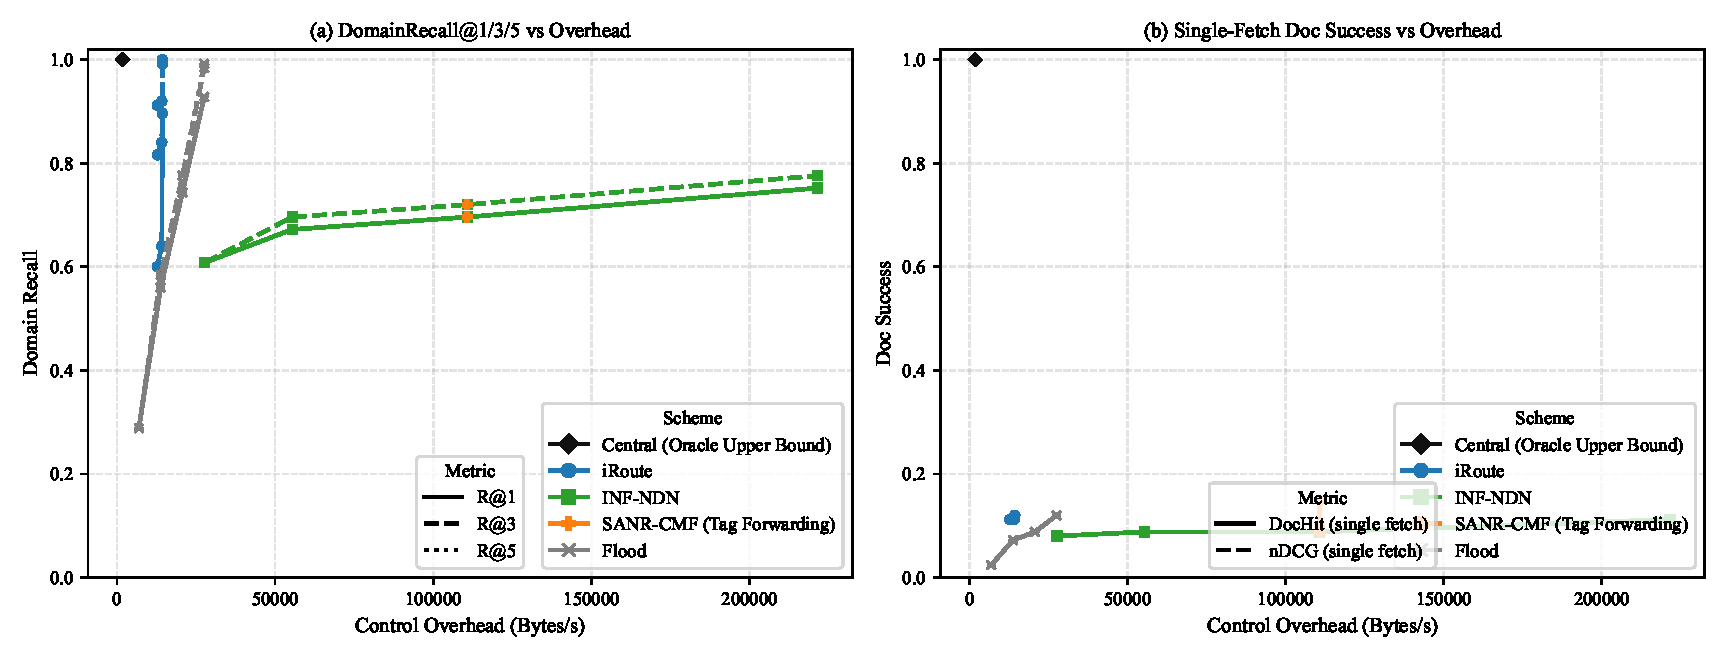
\includegraphics[width=0.92\linewidth]{figs/fig1_accuracy_overhead.pdf}
    \caption{Accuracy versus control overhead in bytes per second.}
    \label{fig:accuracy_overhead}
\end{figure}

% claim-id: eval-correctness-bounded-advertisements
This experiment isolates how bounded advertisements shape correctness.
Increasing $M$ expands centroid coverage and generally improves domain-level coverage, at the cost of higher control overhead.
Flooding provides a high-recall reference by design, while Tag-FIB is constrained by its fixed vocabulary and fails when queries require fine-grained constraints beyond tag resolution.
The centralized-directory curve is interpreted only as an oracle upper bound.
Exact-NDN provides a syntactic reference that is not designed to resolve intent queries.
In the current repository, Fig.~\ref{fig:accuracy_overhead} is regenerated from the cache-disabled paper-grade accuracy bundle; the separate cache-enabled SANR workflow is kept only as exploratory evidence.

\subsection{Retrieval Latency and Path Efficiency}
\label{sec:eval_latency}

% claim-id: eval-latency-selective-probing
We measure end-to-end retrieval time from the instant a consumer issues an intent query to the time it receives the first relevant Data packet.
Fig.~\ref{fig:retrieval_cdf} reports the retrieval time distribution across the query workload.

\begin{figure}[t]
    \centering
    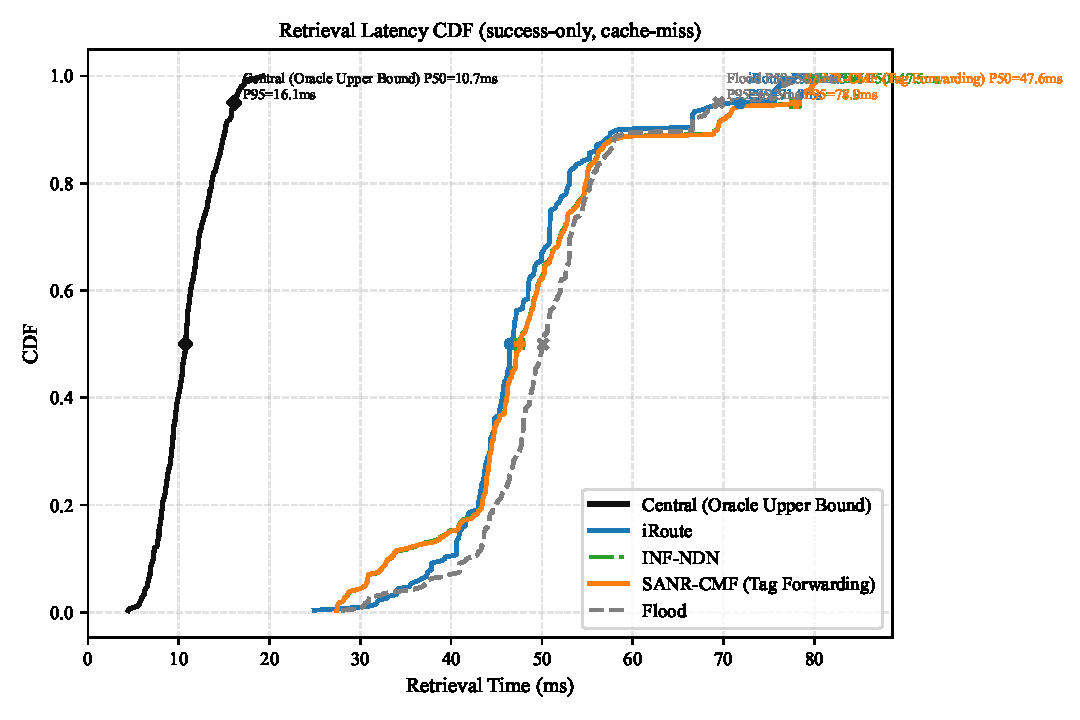
\includegraphics[width=0.92\linewidth]{figs/fig2_retrieval_cdf.pdf}
    \caption{Retrieval time distribution across the query workload.}
    \label{fig:retrieval_cdf}
\end{figure}

Latency reflects both the discovery path and the second-stage fetch.
Selective probing reduces unnecessary network traversal compared to flooding, but it may incur additional retries when semantic confidence is low or when relevance is distributed across multiple domains.
In the current repository, Fig.~\ref{fig:retrieval_cdf} is regenerated from the same cache-disabled paper-grade bundle, so the plotted CDF should be read as routing-only evidence rather than a cache-participation artifact.
Exact-NDN remains a syntactic reference rather than an apples-to-apples intent-discovery baseline when stronger naming knowledge is assumed.
To complement time-based measurements, we report path efficiency using hop count.
Fig.~\ref{fig:hop_load} reports average hop count as offered query load increases, which stress-tests whether selective probing keeps traffic localized and whether queueing and retransmissions inflate effective path length under load.

\begin{figure}[t]
    \centering
    
\includegraphics[width=0.92\linewidth]{figs/fig3_hop_load.pdf}
    \caption{Average hop count versus offered query load.}
    \label{fig:hop_load}
\end{figure}

\subsection{Control-Plane State and Traffic Scaling}
\label{sec:eval_scalability}

% claim-id: eval-scalability-bounded-state
The primary design objective of \sysname{} is bounded routing state as the number of objects and domains grows.
We scale the number of domains while holding the per-domain advertisement budget $M$ fixed, and measure the control-plane state visible at an ingress router.
Fig.~\ref{fig:state_scaling} reports LSDB records and induced forwarding entries as a function of the number of domains.

\begin{figure}[t]
    \centering
    
\includegraphics[width=0.92\linewidth]{figs/fig4_state_scaling.pdf}
    \caption{Control-plane state scaling with the number of domains.}
    \label{fig:state_scaling}
\end{figure}

With a hard budget of $M$ centroids per domain, the expected scaling at ingress is proportional to $|\mathcal{D}|\cdot M$, while local domain state remains bounded by design.
We do not interpret Exact-NDN as a directly comparable state baseline in this figure, because stronger a priori name knowledge changes the comparison target away from intent-driven discovery.
We also report control traffic as bytes per second in Fig.~\ref{fig:accuracy_overhead}.
In the final version, we decompose control traffic into steady-state refresh, burst traffic during updates, and query-driven probe traffic, to identify the dominant contributor under each regime.

\subsection{Robustness Under Churn and Failures}
\label{sec:eval_robustness}

% claim-id: eval-robustness-recovery
IoT deployments face frequent churn and network failures.
We evaluate robustness under three disruption models: churn that changes producer availability, link failures in the backbone, and domain failures that render an entire domain unreachable.
Fig.~\ref{fig:recovery} plots domain-hit rate over time for these scenarios and reports $t_{95}$ recovery time relative to the pre-event domain-hit baseline.

\begin{figure}[t]
    \centering
    \begin{subfigure}[t]{0.32\linewidth}
        \centering
        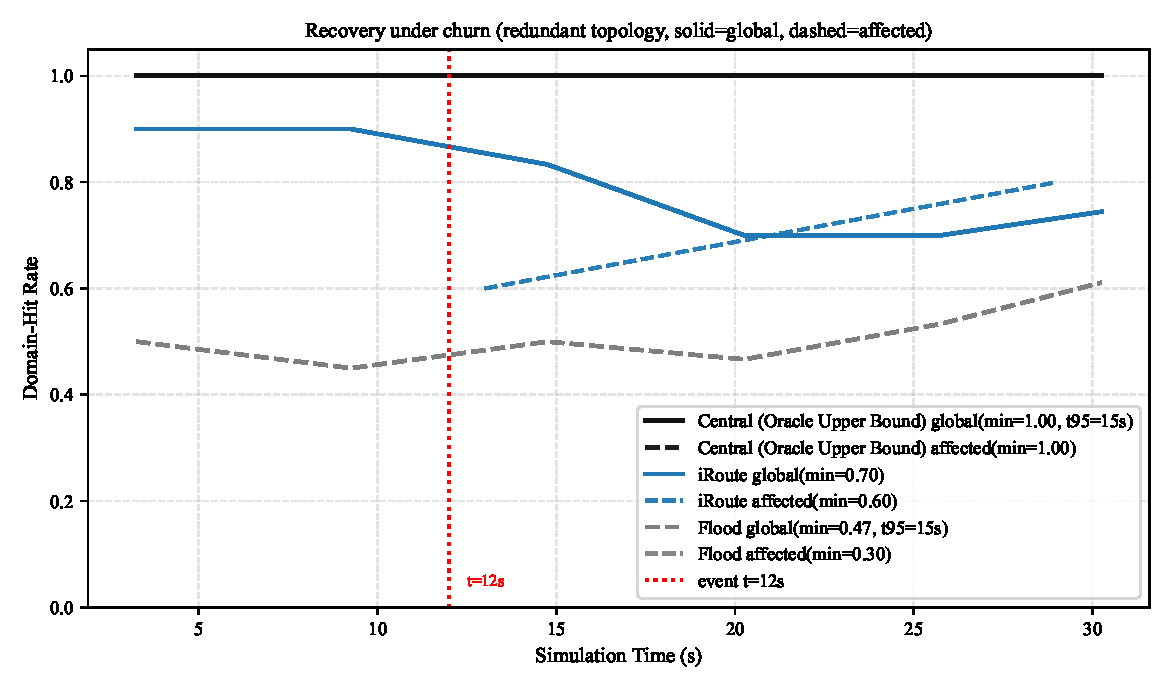
\includegraphics[width=\linewidth]{figs/fig5_recovery_churn.pdf}
        \caption{Churn}
    \end{subfigure}\hfill
    \begin{subfigure}[t]{0.32\linewidth}
        \centering
        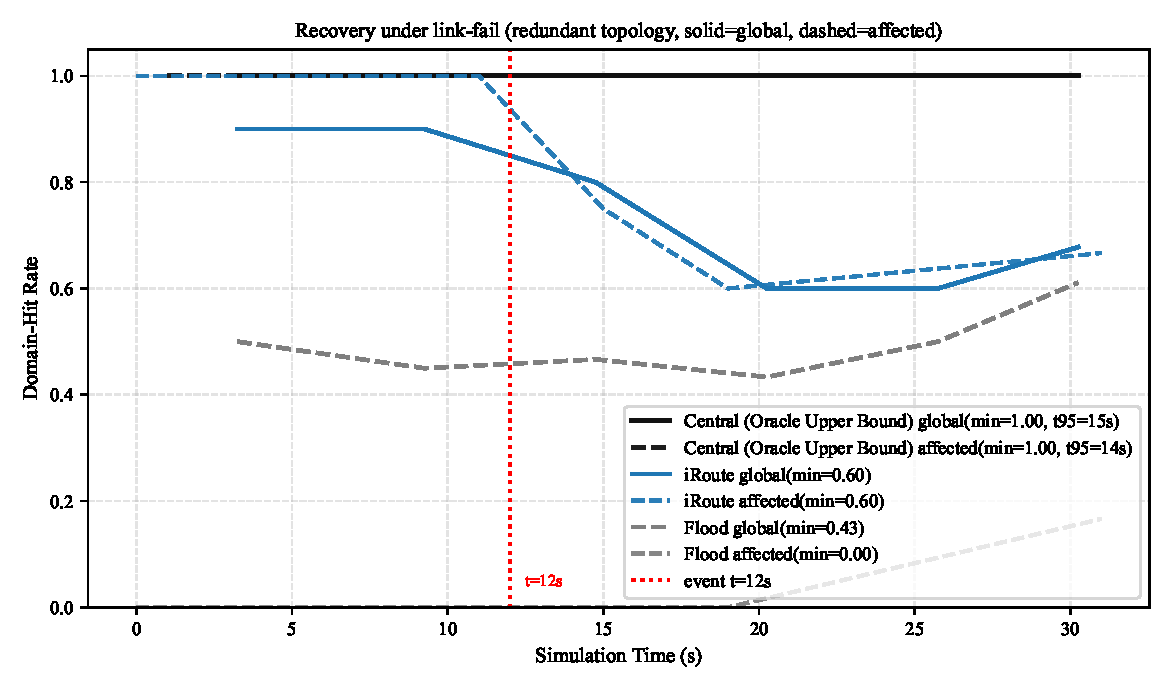
\includegraphics[width=\linewidth]{figs/fig5_recovery_link-fail.pdf}
        \caption{Link failure}
    \end{subfigure}\hfill
    \begin{subfigure}[t]{0.32\linewidth}
        \centering
        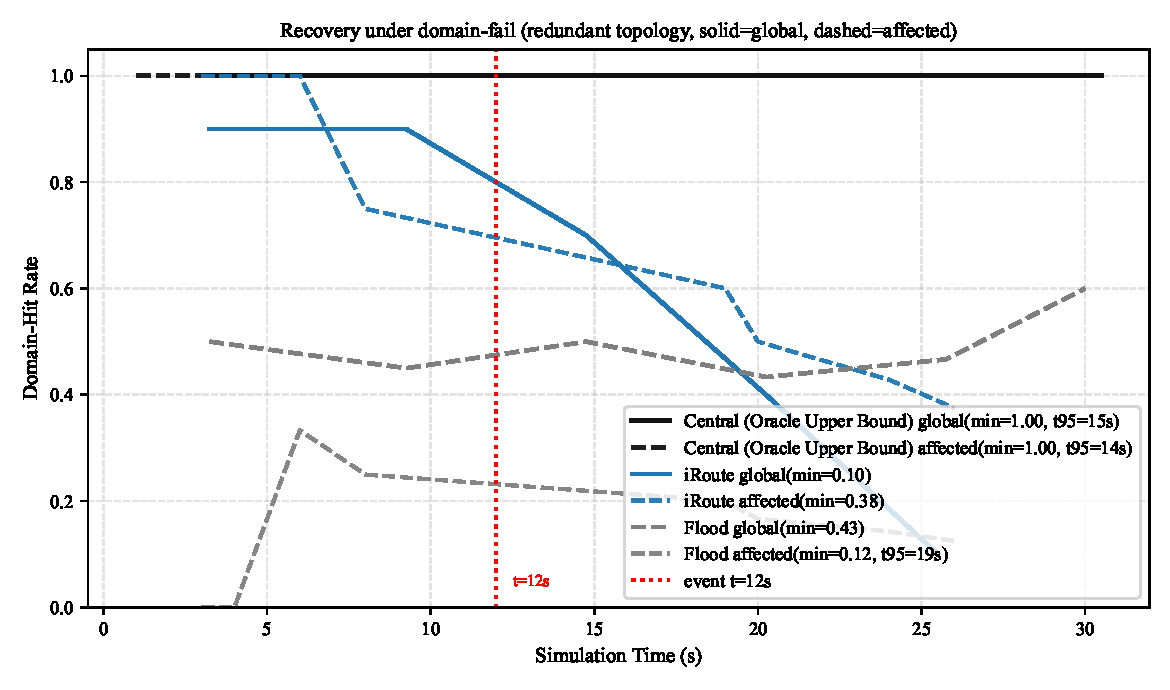
\includegraphics[width=\linewidth]{figs/fig5_recovery_domain-fail.pdf}
        \caption{Domain failure}
    \end{subfigure}
    \caption{Domain-hit rate over time under churn and failures.}
    \label{fig:recovery}
\end{figure}

This section highlights how quickly semantic routing returns to a stable operating point after disruption.
Churn tests whether domains can refresh advertisements without inducing sustained control-plane overload.
Link failures test whether discovery can reroute and maintain acceptable domain-level resolution when shortest paths disappear.
Domain failures test whether the system can avoid repeatedly probing unreachable domains and whether fallback strategies degrade gracefully.

\subsection{Discussion and Lessons}
\label{sec:eval_discussion}

When object-level recall is low, failures typically fall into two categories.
The first category is domain misrouting, in which discovery selects domains without relevant objects.
The second category is intra-domain mismatch, in which discovery reaches a relevant domain but the domain returns a non-relevant canonical name under the current ranking or thresholding.
These categories motivate different remedies.
Increasing $M$ improves centroid coverage and reduces domain misrouting, while improving domain-local resolution logic and the construction of object descriptions and queries reduces intra-domain mismatch.

Trace-driven IoT workloads can also be misleadingly easy or hard depending on query diversity and how much semantic information is present in object descriptions.
A paper-grade evaluation should therefore include a controlled template workload to isolate algorithmic behavior and a harder paraphrase and attribute-variation workload to test semantic generalization.
We also report ablations that remove semantic fields from object descriptions to quantify how much semantics, rather than topology, drives routing decisions.

Finally, our implementation uses offline embeddings and centroid generation, which is appropriate for controlled evaluation but understates the compute cost of continuous updates.
To address this limitation, we add a micro-benchmark reporting embedding and centroid update latency and amortized control traffic per update.
Absolute latency depends on topology and link delays, so our claims emphasize relative comparisons across methods under identical settings.



% =============================================================================
% Restored Full Bibliography
% =============================================================================
\bibliographystyle{IEEEtran}
\begin{thebibliography}{00}

% --- NDN Basics ---
\bibitem{ndn}
L.~Zhang et al., ``Named Data Networking,'' ACM SIGCOMM CCR, vol. 44, no. 3, pp. 66--73, 2014.

\bibitem{ndn_forwarding}
H.~Yi et al., ``A Case for Stateful Forwarding Plane,'' Computer Communications, vol. 36, no. 7, pp. 779--791, 2013.

% --- Routing Protocols (Syntactic) ---
\bibitem{nlsr}
A.~Hoque et al., ``NLSR: Named-data Link State Routing,'' in Proc. ACM ICN, 2013.

\bibitem{distance_vector}
J.~Wang, R.~Wakikawa, and L.~Zhang, ``Distance Vector Routing for Named Data Networking,'' in Proc. IEEE ICNP, 2014.

\bibitem{ondemand}
O.~Ascigil et al., ``On-Demand Routing for Scalable Name-Based Forwarding,'' in Proc. IFIP Networking, 2018.

\bibitem{panini}
T.~Wirtgen et al., ``The Case for PANINI: A Partial and Adaptive Name Information in Network Intermediaries,'' in Proc. IFIP Networking, 2018.

% --- Scalability & FIB Optimization ---
\bibitem{cnr}
S.~S.~Adhatarao et al., ``CNR: Content Name Resolution in Information Centric Networks,'' in Proc. IEEE GLOBECOM, 2016.

\bibitem{samba}
A.~Esmaeili and A.~Mtibaa, ``SAMBA: Scalable Approximate Forwarding For NDN Implicit FIB Aggregation,'' arXiv preprint arXiv:2409.19154, 2024.

\bibitem{scalable_fib_icn15}
T.~Song, H.~Yuan, P.~Crowley, and B.~Zhang, ``Scalable Name-based Packet Forwarding: From Millions to Billions,'' in Proc. ACM ICN, 2015.

\bibitem{scalable_pit_infocom14}
H.~Yuan and P.~Crowley, ``Scalable Pending Interest Table Design: From Principles to Practice,'' in Proc. IEEE INFOCOM, 2014.

\bibitem{enhancing_forwarding_ancs17}
H.~Yuan, P.~Crowley, and T.~Song, ``Enhancing Scalable Name-based Forwarding,'' in Proc. ACM/IEEE ANCS, 2017.

\bibitem{ptcam_sigcomm25}
T.~Song, T.~Li, and Y.~Yang, ``PtCAM: Scalable High-Speed Name Prefix Lookup using TCAM,'' in Proc. ACM SIGCOMM, 2025.

% --- Geometric / Hash-based Routing ---
\bibitem{hyperbolic}
M.~Bogu{\~n}{\'a} et al., ``Hyperbolic Geometry of Complex Networks,'' Physical Review E, vol. 82, 2010.

\bibitem{muca}
C.~Ghasemi et al., ``MUCA: New Routing for Named Data Networking,'' in Proc. IFIP Networking, 2019.

\bibitem{distance_info}
S.~K.~Fayazbakhsh et al., ``Name-Based Content Routing in Information Centric Networks Using Distance Information,'' in Proc. ACM ICN, 2013.

\bibitem{bloom}
S.~Rhea et al., ``Bloom Filters in P2P,'' in Proc. ACM SIGCOMM, 2001.

% --- Semantic & Intelligent Routing ---
\bibitem{inf_ndn_iot}
M.~B.~M.~Kamel et al., ``INF-NDN IoT: An Intelligent Naming and Forwarding,'' IEEE Access, vol. 11, 2023.

\bibitem{fuzzy_forwarding}
K.~Chan et al., ``Fuzzy Interest Forwarding,'' in Proc. ACM ICN, 2017.

\bibitem{semantic_addressing}
D.~Trossen et al., ``Design Considerations for Semantic-based Routing,'' in Proc. IEEE ICCCN, 2012.

\bibitem{ndn_iot_journal}
W.~Shang et al., ``Named Data Networking of Things,'' IEEE Internet of Things Journal, 2016.

\bibitem{p4_ml_infocom19}
Z.~Xiong et al., ``In-network Machine Learning with P4,'' in Proc. IEEE INFOCOM, 2019.

% --- NLP & Embeddings ---
\bibitem{sbert}
N.~Reimers and I.~Gurevych, ``Sentence-BERT: Sentence Embeddings using Siamese BERT-Networks,'' in Proc. EMNLP, 2019.

\bibitem{jl_lemma}
W.~B.~Johnson and J.~Lindenstrauss, ``Extensions of Lipschitz mappings into a Hilbert space,'' Contemporary Mathematics, vol. 26, 1984.

\bibitem{hnsw}
Y.~Malkov and D.~Yashunin, ``Efficient and Robust Approximate Nearest Neighbor Search using HNSW Graphs,'' IEEE TPAMI, vol. 42, no. 4, 2018.

% --- System Implementation Related ---
\bibitem{li2024istack}
T.~Li, T.~Song, and Y.~Yang, ``iStack: A General and Stateful Name-based Protocol Stack for NDN,'' in Proc. USENIX NSDI, 2024.

\bibitem{cluster_caching_access19}
W.~Huang, T.~Song, Y.~Yang, and Y.~Zhang, ``Cluster-based Cooperative Caching with Mobility Prediction in Vehicular NDN,'' IEEE Access, vol. 7, 2019.

\bibitem{nfd_guide}
A.~Afanasyev et al., ``NFD Developer's Guide,'' NDN Technical Report NDN-0021, 2018.

\bibitem{ndnsim}
S.~Mastorakis et al., ``ndnSIM 2.0: A new version of the NDN simulator for NS-3,'' NDN Technical Report NDN-0028, 2015.

\bibitem{rocketfuel}
N.~Spring, R.~Mahajan, and D.~Wetherall, ``Measuring ISP Topologies with Rocketfuel,'' in Proc. ACM SIGCOMM, 2002.

\bibitem{amadeo2025saf}
M.~Amadeo, S.~Serrano, A.~Molinaro, M.~Nitti, and G.~Ruggeri, ``Enhancing IoT Service Discovery through Semantic Name-based Forwarding,'' IEEE Internet of Things Magazine, early access, 2025, doi:10.1109/MIOT.2025.3587052.
\bibitem{antunes2022context}
M.~Antunes, J.~Quevedo, D.~Gomes, and R.~L.~Aguiar, ``Improve Contextual IoT Service Discovery with Semantic Models,'' in Proc. IEEE FiCloud, 2022, doi:10.1109/FiCloud57274.2022.00038.
\bibitem{dt_vndn_semantic}
M.~Amadeo, C.~Campolo, S.~Serrano, A.~Molinaro, and G.~Ruggeri, ``DT-assisted Vehicular Crowdsensing through Semantic-aware NDN,'' in Proc. IEEE Mediterr. Conf. Commun. Netw. (MeditCom), 2025, doi:10.1109/MeditCom64437.2025.11104444.
\bibitem{grewe2018sodi}
D.~Grewe, M.~Wagner, S.~Schildt, A.~Nordmann, and J.~Laverman, ``Towards Semantic Object Discovery for Vehicular Named Data Networks,'' in Proc. IEEE VTC Spring, 2018, doi:10.1109/VTCSpring.2018.8417783.
\bibitem{sanr_cmf}
G.~M.~Raza, I.~Ullah, M.~N.~Ali, and B.-S.~Kim, ``SANR-CMF: Semantic-Aware Naming Resolution and Cache Management Framework in Information-Centric Network for Internet of Things,'' IEEE Internet of Things Journal, vol.~12, no.~17, pp.~35447--35463, 2025, doi:10.1109/JIOT.2025.3578699.
\bibitem{iscc}
G.~M.~Raza, T.~T.~Sar{\i}, G.~Secinti, K.~Aurangzeb, M.~N.~Ali, and B.-S.~Kim, ``ISCC: Intelligent Semantic Caching and Control for NDN-Enabled Industrial IoT Networks,'' IEEE Access, vol.~13, 2025, doi:10.1109/ACCESS.2025.3614984.
\bibitem{semantic_name_dist}
G.~M.~Raza et al., ``Semantic-Driven Intelligent Name Distribution \& Retrieval for Named Data Networking,'' in Proc. IEEE SmartNets, 2025, doi:10.1109/SmartNets65254.2025.11106877.

\bibitem{hybrid_iot_naming}
B.~Nour, K.~Sharif, F.~Li, et~al.,
``A unified hybrid information-centric naming scheme for IoT applications,''
\emph{Computer Communications}, vol.~150, pp.~103--114, 2020.

\bibitem{semantic_name_forwarding_iotmag25}
M.~Amadeo, A.~Campolo, and A.~Molinaro,
``Enhancing IoT Service Discovery through Semantic Name-based Forwarding,''
\emph{IEEE Internet of Things Magazine}, 2025, doi: 10.1109/MIOT.2025.3587052.

\bibitem{sanr_cmf}
G.~M.~Raza, I.~Ullah, M.~Nadeem~Ali, and B.-S.~Kim,
``SANR-CMF: Semantic-Aware Naming Resolution and Cache Management Framework in Information-Centric Network for Internet of Things,''
\emph{IEEE Internet of Things Journal}, vol.~12, no.~17, pp.~35447--35464, Sep.~2025, doi: 10.1109/JIOT.2025.3578699.

\bibitem{antunes_ficloud2022}
M.~Antunes, R.~C.~Oliveira, J.~L.~Fiuza, and R.~G.~Couto,
``Improve Contextual IoT service discovery with semantic models,''
in \emph{Proc. 9th Int. Conf. on Future Internet of Things and Cloud (FiCloud)}, 2022, doi: 10.1109/FiCloud57274.2022.00038.


\end{thebibliography}



\end{document}
